\documentclass{book}
\usepackage{verbatim}
\usepackage{graphicx}
\usepackage{hyperref}
\author{Bart Vermeulen}
\title{ADCPtools}
\newcommand{\funcdef}[1]{\vspace{1pc}\noindent\framebox[\linewidth]{#1}\vspace{1pc}}

\begin{document}
	\maketitle

	\chapter{Introduction}

	\chapter{Reading data}

	\chapter{Low level processing}

	\chapter{Transect data processing}


	Repeat transect can be processed with the function \verb#procTrans.m#. 

	\funcdef{msh=procTrans(adcp.tid)}
	
	This functions accepts two inputs:
	\begin{itemize}
		\item An ADCP structure \verb#adcp# read with \verb#readDeployment.m#.
		\item A transect ID matrix \verb#tid#. 
	\end{itemize}
	\verb#tid# is a matrix of integral numbers with as many columns as ensembles in \verb#adcp# and as many rows as cross-sections you want to process. Any non-zero number at \verb#(i,j)# indicates that the \verb#j#-th ensemble is part of the \verb#i#-th cross-section. The number itself indicates grouping of the ensembles withing a cross-section. If, for example, in one row we have numbers from \verb#1# to \verb#3#, this indicates that all ensembles with number \verb#1# belong together, like all with number \verb#2#, etc. This allows to group subsets of the data within one cross-section (\autoref{fig:tid})

	\begin{figure}
		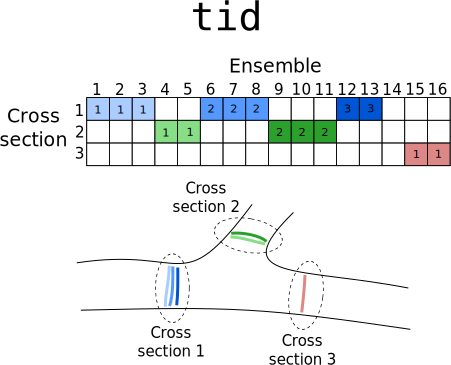
\includegraphics[width=\linewidth]{figures/tid.pdf}
		\caption{Example of a a transect ID matrix. Three cross-section are defined and for each transect different repeat-transect are distinguished. White elements in the matrix indicate zero value.}
		\label{fig:tid}
	\end{figure}


	\chapter{Coupled ADCP processing}

\end{document}